\section{Process}
\subsection{Methodology}
\begin{itemize}
    \item Meetings
    \item Extreme programming
    \item Evaluation Criteria (How were they defined)
\end{itemize}

\subsection{Communication}
Communication with Vixel was done through biweekly status meetings, where they would be briefed on progress, and answer any questions we had related to the direction of the project. Additionally, we would sit in their office when working with the project, allowing for easy communication. Any communication outside of these situations happened through Slack.

\subsection{Pair Programming}
Throughout the project we adopted a pair programming methodology. This was done to ensure that both group members were familiar with the functionality of the code, and to allow us to quickly exchange ideas as to how the functionality could be implemented.

\subsection{High-level Architecture}
\subsubsection{Vixel Proposed Architecture}
Vixel was quite clear on what solution they desired, and presented us with a proposed architecture, seen in figure~\ref{fig:proposed_architecture}. In their proposed architecture the images captured by the camera is sent to a distribution server. From here the video feed is distributed to an clients who \rephrase{are listening for it.}
In the case where a client user clicks to highlight something on their screen, that interaction request is sent to the host through the distribution server.


\begin{figure}
    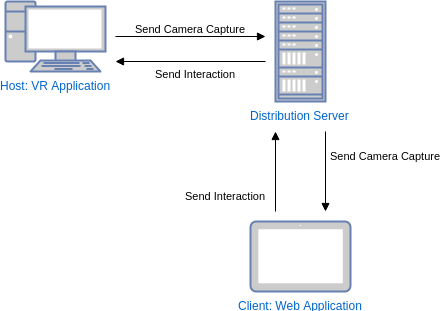
\includegraphics[width=0.8\textwidth]{vixel_stream}
    \caption{Proposed architecture by Vixel}
    \label{fig:proposed_architecture}
\end{figure}

\subsubsection{Our Architecture}
Our final solution is kept quite close to the original solution, with some minor differences. As seen in figure~\ref{fig:our_architecture} rather than only having one distribution server, two cloud servers are used to achieve the desired functionality. The video stream captured by the camera in the host VR application is sent to a dedicated streaming platform, rather than the distribution server. Interactions between the client and the VR application, such as highlighting, is handled through the Photon Cloud. With the move to a dedicated streaming platforms, the client needs to know where to watch the stream. The URL for this stream is also communicated through Photon Cloud.

\paragraph{Justification}
Splitting the distribution server into two separate pieces allowed us to better focus on combining existing solutions to allow us to get a functioning proof of concept faster. Having a distribution server would require us to set up a basic streaming platform. The distribution server would also need functionality to allow it to speak to both the host side Unity VR application and the client web application. Such a solution would require us to satisfy potentially complex networking protocols. This was something we neither had time, nor competence to do.

\begin{figure}
    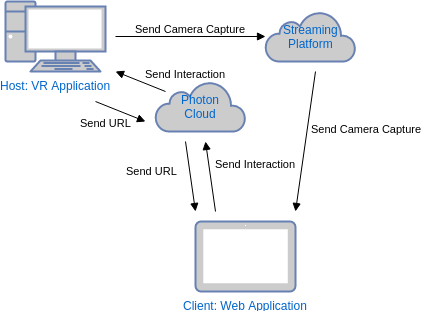
\includegraphics[width=0.8\textwidth]{our_stream}
    \caption{Final Architecture}
    \label{fig:our_architecture}
\end{figure}

\subsection{Technology Assessment and Component Architecture}
* What does this section contain?
    * What our assessment framework was
    * Per component
        * The description of the component, 
        * the alternative solutions we looked at, their strengths and weaknesses, 
        * what our final solution ended up implementing and why.

\subsubsection{Assessment Framework}
* How did we assess technology?
    * Gauging our first impressions on various technology
    * Setting up a set of criteria
    * Each criteria has a importance multiplier from 1-5, higher means more important
    * Each alternative solution is then given a score from 0-9 for each criteria
    * A total sum is then calculated per solution where the score of each criteria is combined with the respective importance multiplier. 
    * The solutions that then had the highest scores were the ones we would discuss further and potentially choose for usage.

* We are only listing the solutions we were able to think of and find. There may of course be additional solutions available that we missed. 
* We handled the technology assessment with the original model/architecture in mind, but the final architecture ended up being slightly different due to our final choice of technologies and the fact that we grew more familiar with the concept of streaming. 

\subsubsection{Host - Image Capture} % FFMPEGOut in combination with FFMPEG. Some modified source code for optimization and repurposing for streaming
Image capturing is a subcomponent of the host component where the goal is to capture images at a set time interval from a camera that exists in Unity. The captured images then need to be encoded to a video format in order for streaming to be possible. As far as technology assessment is concerned, we primarily looked at the actual problem of capturing images first and foremost as it was the most pressing issue in relation to performance. The solution alternatives we looked at is as follows:
\paragraph{Native C++ Plugin, using OpenGL access to acquire framebuffer}
        * Description
            \todo{cite/footnote documentation}
            * Unity has support for native C++ plugins through the use of DLL files. This allows writing native C++ code while having full access to the rendering pipeline. By having access to the pipeline, we could access the framebuffer directly and acquire the image data from there.   
        * Strengths
            * Huge amounts of control to do almost everything we want 
            * High performance potential
        * Weaknesses
            * Need to restart Unity every time we want to reload the plugin
            * Fairly high code complexity
            * Understanding of Unity's rendering pipeline is required
\paragraph{RockVR Video Capture}
        * Description
            \todo{cite/footnote}
            * RockVR is a free plugin from the Unity Asset Store that allows for plug and play video capture functionality. 
        * Strengths
            * Seems simple to use. 
        * Weaknesses
            * Performance is not good enough
            * Hard to understand how to replace video file encoding to actual real time encoding.
            * Licensing is unknown. 
            * Paid version is required for more functionality. 
\paragraph{Naive implementation using RenderTexture in Unity}
        * Description
            \todo{cite/footnote documentation}
            * The simplest solution is to use Unity's RenderTexture components and copy pixel data directly from a camera view to a texture. 
        * Strengths
            * Easiest solution to prototype
            * Very low code complexity
        * Weaknesses
            * Very mediocre performance
\paragraph{Optimized Naive implementation}
        * Description
            \todo{cite post}
            * Google's Tiltbrush developers posted a blog post where they went through a high level description of how they optimized their video capture functionality in tiltbrush to support real time VR video capture. It might thus be possible to retrace the steps mentioned in the post to create an optimized naive implementation as the blog post starts with it as a base. 
        * Strengths
            * Supposedly high enough performance for real time video capture, even in VR.
            * Written by google's tiltbrush developers so the claims and data of the blog should be fairly valid. 
        * Weaknesses
            * Would actually require implementation of a solution that is explained at a high level in a blog post. Can be hard with limited knowledge on the topic. 
\paragraph{Unity Generic Frame Recorder}
        * Description
            \todo{cite/footnote}
            * Unity offers a open source video capturing plugin which contains a large amount of functionality. 
        * Strengths
            * Fairly large and extensible plugin made by Unity themselves for recording. 
            * Pretty well documented
            * Open source
        * Weaknesses
            * The code base is a bit too big and complex for our use case. This makes it hard to actually modify and extend the code to fit our needs 
            * General performance did not seem satisfactory. 
\paragraph{Using the AsyncGPUReadback from the latest Unity version}
        * Description
            \todo{cite/footnote documentation?}
            * Unity 2018 added the possibility of asynchronous readback from the GPU which in general should allow for high performance fetching of data. 
        * Strengths
            * Supposedly allows quick and instant readback from the GPU without stalling the rendering pipeline like standard usage of RenderTexture would. 
        * Weaknesses
            * Experimental technology that might be removed from Unity later
            * No actual open source implementations that handle video recording in a high performance manner. Attempting a quick prototype with this resulted in lower performance than even the naive implementation. This primarily came from the fact that we could not properly send the data directly to FFmpeg as it had to be converted to a supported format first. We could not find a efficient enough data conversion to actually make use of this. 
\paragraph{FFmpegOut}
        * Description
            \todo{cite/footnote}
            * FFmpegOut is a open source plugin for Unity that handles video capturing using the FFmpeg library as a video encoder. 
            * Note: We found this after prototyping with the rest of available solutions while studying how to handle video encoding. 
        * Strengths
            * Best performance
            * Gives access to a powerful industry standard library directly in C\#
            * Open Source
            * Relatively small code base so it is easy to keep track of everything and modify the code. 
        * Weaknesses
            * Will require time to learn how to use a very big library to actually do what we want. 
            * The FFmpeg pipe from the source code is not perfectly robust so the recording might suddenly stop working if the window is not in focus for a few seconds. 
\paragraph{Final Choice of Solution}
    * Given that performance was a priority for this case, we prototyped all of the available ready made solutions in combination with the basic naive approach.
    * The majority of these solutions had many oddities and very high performance costs
    * Furthermore, they primarily saved data to files, which is not needed for our case where we want to stream data in real time. 
    * We finally chose FFmpegOut as it allowed us to handle real time encoding of raw image data and stream it using the rtmp protocol. It also had the best performance of the alternatives, albeit not optimal. The fact that the code is open source also allows us to modify the code to suit our needs. 
    * Using the other solutions would require us to at the very least find some means to encode video, but since FFmpegOut provided us access to the FFmpeg library in C\#, this increased the value significantly. 
    
    * The final solution uses a modified version of FFmpegOut where: 
        * we have optimized the performance to no longer force vsync when capturing frames and instead sampling at set time intervals. 
        * Instead of encoding and saving the raw image data to a video file, we have also entirely replaced the FFmpeg command arguments to allow for streaming to both youtube and twitch. 
    

\subsubsection{Host - Data Transfer} % FFMPEG
    * This is a subcomponent of the host side where the main goal is to take the encoded video data and stream it to a distribution server.
    

\paragraph{Native C++ Plugin Using Boost}
    * Description
        * Similar to image capturing we considered using a Native C++ Plugin for Unity that could take the video data and use the networking components of the Boost library to transfer data to the distribution server.  
    * Strengths
        * Access to sockets gives a lot of control
    * Weaknesses
        * The need to make our own protocols
        * Boost is a big library which makes build times a problem
        * Again, Unity requires a reload for every reload of the plugin. 
\paragraph{Unity's Transport Layer}
    * Description
        * While Unity offers a high level network API which primarily is focused around networking for games it also offers a lower level API called the Unity Transport Layer. This API should provide enough functionality to facilitate the process of data transfer to a receiving distribution server.
    * Strengths
        * Allows us to work directly in Unity, reducing dependencies on other libraries. 
        * General reliability should be good as all of Unity's networking functionality is built on top of this API.
    * Weaknesses
        * Documentation is not very comprehensive
        * Will probably have to write our own data transfer protocol. 
        * Limited familiarity with the technology makes it hard to prototype with. 
\paragraph{Photon}
    * Description
        * The Photon Cloud Service offers a Unity API for networking which we potentially could use for transferring data as it supports communication between very many different platforms. 
    * Strengths
        * Allows us to use technology that Vixel already makes use of, potentially easing integration for future development. 
        * Fairly easy to use Unity API.
        * Could allow for using the same technology in multiple places like communication between clients/host
    * Weaknesses
        * Photon is not really built for transfer of video data
        * It will be costly/expensive to actually get the right performance we want from the cloud service.
\paragraph{FFmpeg}
    * Description
        * \todo{FFmpeg library description}
    * Strengths
        * Direct support for the RTMP protocol which is used for video streaming
        * Primary focus is manipulation of video files. 
        * Very well documented
        * Can also take care of video encoding. 
    * Weaknesses
        * The library is fairly big so it can take a little bit of time to learn what we need. 

\paragraph{Final Choice of Solution}
    * In general, it was hard to make a choice for this component as we had no prior experience with large scale data transfer.
    * Originally we had decided to go for using the Unity Transport Layer as a means to transfer data.
        * The reason for this is that we primarily wanted to work in Unity if possible to reduce overhead. 
    * We also considered Photon, but discussion with Vixel provided us with the information that Photon is not that efficient at transferring large amounts of data like with videos at a time
    * After finding the FFmpegOut plugin for video capture, we found out that FFmpeg also supports video streaming. 
        * FFmpeg is generally very well documented and used in popular streaming software like Open Broadcasting Software. 
        * Using it also means we can use a piece of technology to take care of two things at once, which lessens the complexity of the code base and allows for quicker prototyping. Speed of prototyping was a very important factor for the development of this project as we had rather limited time to actually make something. 
        * FFmpeg is also primarily focused around working with video files which also provides a very optimized environment as far as latency is concerned. 


\subsubsection{Host/Client Communication} % Photon
    * This component consists of facilitating the communication between the host and the clients. This includes distributing stream URLs and interaction from the client side to send screen click events back to the host
    * In general, the aforementioned alternative solutions outside of C++ with Boost and FFmpeg could be used for communication between clients and host, but we have to consider additional factors when interacting between different platforms as the client will be served through a web page. 
        * Basically cross platform priority. 
        * Boost is irrelevant as we are dealing with Javascript
    
\paragraph{Unity's Transport Layer}
    * Strengths
        * A lot of control in terms of how communication is handled.
    * Weaknesses
        * Can potentially force us to use Unity on the client side which might result in less maintainable and extensible code. Ideally we would like to have components be as interchangeable as possible.  
        * General complexity of low level networking
        * We do not need all the control to simply transfer text/some positions between host and clients. 
\paragraph{Photon}
    * Strengths
        * Very easy to set up.
        * Already used by Vixel to some extent. 
        * Full cross platform support. Can be used with Unity, but will also support a full javascript client.
    * Weaknesses
        * Free service provides limited functionality 

\paragraph{Final Choice of Solution}
    * Ultimately we went with Photon for communication as it was very easy to set up for prototyping and the additional cross platform support allowed us to deal with potentially different technologies on the client side outside of Unity if necessary. 

\subsubsection{Server - Stream Distribution} % Youtube, Twitch, Mixer, Self made streaming solution
    * The encoded video data needs to be sent to a type of distribution server which takes the data and streams/distributes it to all connected clients in the form of a livestream.
        * Because the host should not be using additional bandwidth other than sending the video data to this server. 
\paragraph{Self-Made streaming platform}
    * Description
        * As the name implies, this solution would require us to make our own streaming platform which distributes the stream data to all clients. 
    * Strengths
        * Full control over this component of the solution
        * Potentially no expenses
    * Weaknesses
        * We will have to host the server locally which limits bandwidth throughput
        * Complexity of creating a streaming platform from scratch without any prior experience is very large. 
\paragraph{Making use of existing stream middleware}
    * Description
        * There is streaming middleware out there which could be used to create our own streaming platform in a quicker manner. \todo{add examples}
    * Strengths
        * Potential cloud distribution should make bandwidth less of a problem.
        * A fair amount of control is still given in relation to how the server distributes streaming. 
    * Weaknesses
        * There are usually expenses involved in both the platform and cloud hosting.
        * Unknown latency between host and client. 
\paragraph{Making use of streaming platforms like Youtube and Twitch}
    * Description
        * The final alternative would be to make use of existing streaming platforms like Youtube/Twitch and embed their stream player into our website with input functionality overlayed on top of the player. 
    * Strengths
        * Completely free
        * High performance distribution of streams which should result in minimal latency
        * Easier and faster to prototype with
    * Weaknesses
        * Technically using the platforms for purposes they are not made for.
            * Point 5.G in the youtube terms. 
                * Not sure if we are breaking this rule, but we are blocking the possibility of pausing the stream.  
                * And we are building functionality on top of it.
        * Very limited control over the platform. 
\paragraph{Final Choice of Solution}
    * Our final choice here ultimately ended up being using Twitch and Youtube as our streaming platforms. The rationale behind the choice is
        * we simply did not have the time and resources available to make our own streaming platform
        * we do not want to spend money on the solution for a prototype
        * latency is of high importance so we went with the best free solution that also provided the minimal latency. 
    * The loosely coupled architecture of the project makes it easy to potentially replace what we used with another platform.

\subsubsection{Client} % Unity Overlay HTML 5, Moving to pure javascript, Remember: glorious html overlay hack
    * Finally, we have the client component which plays the livestream while also listening for mouse clicks which are sent back to the host. 
    * Limited options as no installation was a requirement.
\paragraph{Pure Javascript Client}
    * Description
        * A pure Javascript Client could make use of the Photon Javascript API for communication between clients.
        * Playing the livestream could be handled with a embedded player and a invisible overlay to handle mouse clicks(using base Javascript input functionality). 
    * Strengths
        * Pure cross platform functionality. 
        * Very lightweight. 
    * Weaknesses
        * Unfamiliarity with Javascript decreases productivity. 
        * Photon's Javascript API has limited documentation
\paragraph{HTML5 Youtube Player With Unity WebGL Overlay}
    * Description
        * Another option is to have a Unity interface as the overlay over the stream player. 
        * Using Javascript plugins for Unity to communicate between Unity and Javascript. 
        * Unity can take care of input handling. 
    * Strengths
        * Rapid prototyping due to more familiar technology
        * Reducing complexity by using some of the same technology on both host and client side.
        * Photon support is better using Unity. 
    * Weaknesses
        * Unity's WebGL support is still in an early phase. How well it runs on a mobile or tablet is unknown. 
        * A rather heavy solution. 
        * Takes a lot of time to build with WebGL
            * Not robust at all, fails randomly during builds
\paragraph{Final Choice of Solution}
    * Final choice ended up being the Unity WebGL even though the Javascript option technically is a bit better.
        * The rationale behind this was to get the prototype done as quick as possible for the sake of testing and optimizing. 
        * We started some work on the Javascript side after finishing Unity, but we did not have the time to finish it. 
